% =============================================================================
% Pico Miner -- Memoria del Proyecto
% Acelerador de Mineria Bitcoin basado en FPGA
%
% Asignatura: Diseno de Sistemas Electronicos
% Universidad Politecnica de Cartagena
%
% Autores: Jose David Guerrero Romero
%          Enrique Morales Bermejo
% =============================================================================
\documentclass[12pt,a4paper]{article}

% --- Packages ---
\usepackage[utf8]{inputenc}
\usepackage[T1]{fontenc}
\usepackage[provide=*,spanish]{babel}
\usepackage{geometry}
\usepackage{graphicx}
\usepackage{amsmath,amssymb}
\usepackage{listings}
\usepackage[table]{xcolor}
\usepackage{hyperref}
\usepackage{booktabs}
\usepackage{caption}
\usepackage{algorithm}
\usepackage{algorithmic}
\usepackage{tikz}
\usepackage{fancyhdr}
\usepackage{titlesec}
\usepackage{tabularx}
\usepackage{enumitem}
\usetikzlibrary{shapes,arrows,positioning,fit,calc}

\geometry{margin=2.5cm, top=3cm, bottom=3cm}

% =============================================================================
% Blue-Tone Color Theme
% =============================================================================
\definecolor{darkblue}{RGB}{0,51,102}
\definecolor{medblue}{RGB}{0,82,148}
\definecolor{lightblue}{RGB}{0,120,190}
\definecolor{paleblue}{RGB}{220,235,250}
\definecolor{accentblue}{RGB}{70,130,180}

\definecolor{codebg}{RGB}{245,248,252}
\definecolor{codegreen}{rgb}{0,0.45,0}
\definecolor{codegray}{rgb}{0.5,0.5,0.5}
\definecolor{codeblue}{RGB}{0,51,102}

% --- Hyperlinks ---
\hypersetup{
    colorlinks=true,
    linkcolor=darkblue,
    urlcolor=lightblue,
    citecolor=medblue,
    pdfauthor={Jose David Guerrero Romero, Enrique Morales Bermejo},
    pdftitle={Pico Miner -- Memoria del Proyecto}
}

% --- Section Formatting ---
\titleformat{\section}
    {\normalfont\Large\bfseries\color{darkblue}}
    {\thesection}{1em}{}[\color{medblue}\titlerule]

\titleformat{\subsection}
    {\normalfont\large\bfseries\color{medblue}}
    {\thesubsection}{1em}{}

\titleformat{\subsubsection}
    {\normalfont\normalsize\bfseries\color{accentblue}}
    {\thesubsubsection}{1em}{}

% --- Header/Footer ---
\pagestyle{fancy}
\fancyhf{}
\fancyhead[L]{\small\color{medblue}\textbf{Pico Miner}}
\fancyhead[R]{\small\color{medblue}UPCT -- Dise\~no de Sistemas Electr\'onicos}
\fancyfoot[C]{\small\color{medblue}\thepage}
\renewcommand{\headrulewidth}{0.5pt}
\renewcommand{\headrule}{\hbox to\headwidth{\color{medblue}\leaders\hrule height \headrulewidth\hfill}}
\renewcommand{\footrulewidth}{0.3pt}
\renewcommand{\footrule}{\hbox to\headwidth{\color{paleblue}\leaders\hrule height \footrulewidth\hfill}}

% --- Code listing style ---
\lstdefinestyle{cstyle}{
    backgroundcolor=\color{codebg},
    basicstyle=\ttfamily\footnotesize,
    breaklines=true,
    captionpos=b,
    commentstyle=\color{codegreen},
    keywordstyle=\color{codeblue}\bfseries,
    stringstyle=\color{red!70!black},
    numberstyle=\tiny\color{codegray},
    numbers=left,
    frame=single,
    rulecolor=\color{medblue!40},
    language=C,
    showstringspaces=false,
    tabsize=4
}

\lstdefinestyle{tclstyle}{
    backgroundcolor=\color{codebg},
    basicstyle=\ttfamily\footnotesize,
    breaklines=true,
    captionpos=b,
    commentstyle=\color{codegreen},
    keywordstyle=\color{codeblue}\bfseries,
    frame=single,
    rulecolor=\color{medblue!40},
    language=Tcl,
    showstringspaces=false,
    numbers=none,
    tabsize=4
}

% =============================================================================
% Title Page
% =============================================================================
\begin{document}

\begin{titlepage}
    \begin{center}
        \vspace*{1cm}

        % University bar
        \noindent\colorbox{darkblue}{%
            \parbox{\dimexpr\textwidth-2\fboxsep}{%
                \centering\color{white}\large\bfseries
                \vspace{0.4cm}
                Universidad Polit\'ecnica de Cartagena\\[0.2cm]
                \normalsize Escuela T\'ecnica Superior de Ingenier\'ia de Telecomunicaci\'on\\[0.2cm]
                \normalsize Dise\~no de Sistemas Electr\'onicos
                \vspace{0.4cm}
            }%
        }

        \vspace{2cm}

        % Title block
        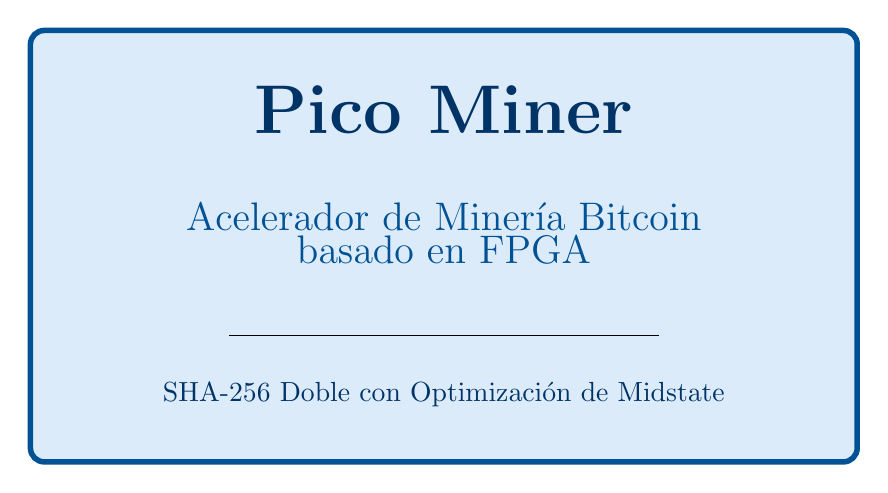
\begin{tikzpicture}
            \node[rectangle, draw=medblue, line width=2pt, inner sep=20pt,
                  rounded corners=5pt, fill=paleblue] (title) {
                \begin{minipage}{0.75\textwidth}
                    \centering
                    {\Huge\bfseries\color{darkblue} Pico Miner}\\[0.6cm]
                    {\Large\color{medblue} Acelerador de Miner\'ia Bitcoin\\
                     basado en FPGA}\\[0.5cm]
                    \rule{0.6\textwidth}{0.5pt}\\[0.4cm]
                    {\normalsize\color{darkblue}
                     SHA-256 Doble con Optimizaci\'on de Midstate}
                \end{minipage}
            };
        \end{tikzpicture}

        \vspace{2cm}

        % Authors
        {\large\color{darkblue}
        \begin{tabular}{rl}
            \textbf{Autores:} & Jos\'e David Guerrero Romero \\
                              & Enrique Morales Bermejo \\[0.5cm]
            \textbf{Plataforma:} & Xilinx Zynq-7020 (ZedBoard) \\[0.3cm]
            \textbf{Herramienta:} & Vivado HLS 2019.1 \\[0.3cm]
            \textbf{Bloque demo:} & Bitcoin Block \#939260 \\[0.3cm]
            \textbf{Fecha:} & Marzo 2026 \\
        \end{tabular}
        }

        \vfill

        % Bottom bar
        \noindent\colorbox{medblue}{%
            \parbox{\dimexpr\textwidth-2\fboxsep}{%
                \centering\color{white}\normalsize
                \vspace{0.3cm}
                Memoria del Proyecto
                \vspace{0.3cm}
            }%
        }
    \end{center}
\end{titlepage}

% =============================================================================
% Table of Contents
% =============================================================================
\tableofcontents
\newpage

% =============================================================================
\section{Introducci\'on}
% =============================================================================

La miner\'ia de criptomonedas es el proceso mediante el cual se verifican las
transacciones y se a\~naden al registro distribuido conocido como \textit{blockchain}.
El reto computacional central se denomina \textbf{Prueba de Trabajo} (\textit{Proof of Work},
PoW): los mineros deben encontrar un valor llamado \textit{nonce} tal que el hash
del bloque de datos cumpla una condici\'on de dificultad --- t\'ipicamente, el hash
resultante debe ser num\'ericamente menor que un valor \textit{objetivo} (\textit{target}).

En Bitcoin, esto implica calcular la funci\'on hash SHA-256 dos veces
(\textit{double SHA-256}) sobre una cabecera de bloque de 80 bytes, iterando
sobre un espacio de nonces de 32 bits. El objetivo de dificultad se ajusta
para que, en promedio, se encuentre un nonce v\'alido cada 10 minutos en toda
la red.

\textbf{Pico Miner} implementa la miner\'ia Bitcoin double-SHA-256 con optimizaci\'on
de midstate, acelerada en una FPGA Zynq-7020 mediante Vivado HLS 2019.1.
La demostraci\'on mina el Bloque 939260 de Bitcoin (4 de marzo de 2026,
dificultad 144.398.401.518.101) desde nonce=0 en aproximadamente 3 minutos,
con retroalimentaci\'on en tiempo real por terminal UART y LEDs del ZedBoard.

% =============================================================================
\section{Fundamentos: Miner\'ia Bitcoin}
% =============================================================================

\subsection{La Blockchain}

Una blockchain es un registro distribuido y de solo escritura, donde cada bloque
contiene:
\begin{itemize}[leftmargin=2em]
    \item Una referencia (hash) al bloque anterior
    \item Un conjunto de transacciones (representadas por la ra\'iz de Merkle)
    \item Una marca de tiempo (\textit{timestamp}) y bits de dificultad
    \item Un valor \textit{nonce}
\end{itemize}

\subsection{Cabecera de Bloque de 80 Bytes}

Cada cabecera de bloque de Bitcoin consta de exactamente 80 bytes (640 bits):

\begin{table}[h]
    \centering
    \caption{Estructura de la cabecera de bloque Bitcoin}
    \rowcolors{2}{paleblue}{white}
    \begin{tabular}{@{}lcl@{}}
        \toprule
        \textbf{Campo} & \textbf{Bytes} & \textbf{Descripci\'on} \\
        \midrule
        Version           & 4  & N\'umero de versi\'on del bloque \\
        Previous hash     & 32 & Hash SHA-256d del bloque anterior \\
        Merkle root       & 32 & Hash de todas las transacciones \\
        Timestamp         & 4  & Marca de tiempo Unix \\
        Bits              & 4  & Representaci\'on compacta del objetivo \\
        Nonce             & 4  & Valor iterado por los mineros \\
        \bottomrule
    \end{tabular}
\end{table}

\subsection{Prueba de Trabajo}

El mecanismo de PoW requiere que:
\begin{equation}
    \text{SHA-256}\bigl(\text{SHA-256}(\text{cabecera\_bloque})\bigr) < \text{objetivo}
\end{equation}

Dado que SHA-256 se comporta como un or\'aculo pseudo-aleatorio, la \'unica forma
de encontrar un nonce v\'alido es mediante \textbf{iteraci\'on por fuerza bruta}:
probando valores de nonce uno por uno hasta cumplir la condici\'on.

\subsection{Ventajas de las FPGAs}

Las FPGAs ofrecen varias ventajas para la miner\'ia PoW:
\begin{itemize}[leftmargin=2em]
    \item \textbf{Paralelismo}: M\'ultiples c\'alculos de hash simult\'aneos en hardware
    \item \textbf{Pipeline}: Las rondas de compresi\'on se pueden segmentar profundamente
    \item \textbf{Eficiencia energ\'etica}: Hardware dedicado es m\'as eficiente que CPUs o GPUs
    \item \textbf{Baja latencia}: Implementaci\'on directa sin overhead de b\'usqueda/decodificaci\'on de instrucciones
\end{itemize}

% =============================================================================
\section{Algoritmo SHA-256}
% =============================================================================

\subsection{Visi\'on General}

SHA-256 (Secure Hash Algorithm, 256 bits) est\'a definido en FIPS 180-4.
Procesa la entrada en bloques de 512 bits (64 bytes), manteniendo un estado
de ocho palabras de 32 bits (256 bits en total) que se actualiza mediante
una funci\'on de compresi\'on de 64 rondas.

\subsection{Relleno del Mensaje}

El mensaje de entrada se rellena hasta ser m\'ultiplo de 512 bits:
\begin{enumerate}[leftmargin=2em]
    \item A\~nadir un bit \texttt{1}
    \item A\~nadir bits \texttt{0} hasta que la longitud sea $\equiv 448 \pmod{512}$
    \item A\~nadir la longitud original del mensaje como un entero de 64 bits en big-endian
\end{enumerate}

Para la cabecera Bitcoin de 80 bytes, el mensaje rellenado tiene 1024 bits
(dos bloques de 512 bits).

\subsection{Funci\'on de Compresi\'on}

Cada bloque de 512 bits se procesa seg\'un el Algoritmo~\ref{alg:sha256compress}.

\begin{algorithm}[H]
    \caption{Compresi\'on SHA-256 (un bloque de 64 bytes)}
    \label{alg:sha256compress}
    \begin{algorithmic}[1]
        \STATE \textbf{Entrada:} Estado $H[0..7]$, Bloque de mensaje $M[0..15]$
        \STATE \textbf{Expansi\'on del calendario de mensajes:}
        \FOR{$i = 0$ \TO $15$}
            \STATE $W[i] \leftarrow M[i]$
        \ENDFOR
        \FOR{$i = 16$ \TO $63$}
            \STATE $W[i] \leftarrow \sigma_1(W[i{-}2]) + W[i{-}7] + \sigma_0(W[i{-}15]) + W[i{-}16]$
        \ENDFOR
        \STATE \textbf{Inicializar variables de trabajo:}
        \STATE $a,b,c,d,e,f,g,h \leftarrow H[0],H[1],\ldots,H[7]$
        \STATE \textbf{64 rondas de compresi\'on:}
        \FOR{$i = 0$ \TO $63$}
            \STATE $T_1 \leftarrow h + \Sigma_1(e) + \text{Ch}(e,f,g) + K[i] + W[i]$
            \STATE $T_2 \leftarrow \Sigma_0(a) + \text{Maj}(a,b,c)$
            \STATE $h \leftarrow g;\; g \leftarrow f;\; f \leftarrow e;\; e \leftarrow d + T_1$
            \STATE $d \leftarrow c;\; c \leftarrow b;\; b \leftarrow a;\; a \leftarrow T_1 + T_2$
        \ENDFOR
        \STATE \textbf{Actualizar estado:}
        \STATE $H[i] \leftarrow H[i] + \{a,b,c,d,e,f,g,h\}$ para $i = 0..7$
    \end{algorithmic}
\end{algorithm}

Las funciones SHA-256 utilizadas son:
\begin{align}
    \text{Ch}(e,f,g)  &= (e \wedge f) \oplus (\neg e \wedge g) \\
    \text{Maj}(a,b,c) &= (a \wedge b) \oplus (a \wedge c) \oplus (b \wedge c) \\
    \Sigma_0(a)        &= \text{ROTR}^2(a) \oplus \text{ROTR}^{13}(a) \oplus \text{ROTR}^{22}(a) \\
    \Sigma_1(e)        &= \text{ROTR}^6(e) \oplus \text{ROTR}^{11}(e) \oplus \text{ROTR}^{25}(e) \\
    \sigma_0(x)        &= \text{ROTR}^7(x) \oplus \text{ROTR}^{18}(x) \oplus \text{SHR}^3(x) \\
    \sigma_1(x)        &= \text{ROTR}^{17}(x) \oplus \text{ROTR}^{19}(x) \oplus \text{SHR}^{10}(x)
\end{align}

\subsection{Doble SHA-256 para Bitcoin}

La miner\'ia Bitcoin calcula:
\[
    \text{hash} = \text{SHA-256}\bigl(\text{SHA-256}(\text{cabecera}_{80\text{B}})\bigr)
\]

El primer SHA-256 procesa la cabecera de 80 bytes (rellenada a 128 bytes = 2 bloques).
El segundo SHA-256 procesa el resultado de 32 bytes (rellenado a 64 bytes = 1 bloque).
Total sin optimizaci\'on: \textbf{3 compresiones} por nonce.

% =============================================================================
\section{Optimizaci\'on de Midstate}
% =============================================================================

\subsection{Idea Clave}

La cabecera de 80 bytes abarca dos bloques de entrada SHA-256:
\begin{itemize}[leftmargin=2em]
    \item \textbf{Chunk 1} (bytes 0--63): versi\'on + hash previo + ra\'iz de Merkle bytes 0--27
    \item \textbf{Chunk 2} (bytes 64--79 + relleno): ra\'iz de Merkle bytes 28--31 + timestamp + bits + \textbf{nonce}
\end{itemize}

Dado que el nonce est\'a en el chunk 2, el estado SHA-256 tras procesar el chunk 1
es \textbf{constante} para todos los intentos de nonce. Este estado intermedio se
denomina \textit{midstate}.

\begin{table}[h]
    \centering
    \caption{Divisi\'on de la cabecera para midstate}
    \rowcolors{2}{paleblue}{white}
    \begin{tabular}{@{}lccl@{}}
        \toprule
        \textbf{Chunk} & \textbf{Bytes} & \textbf{Contenido} & \textbf{Procesado por} \\
        \midrule
        Chunk 1 & 0--63 & version + prev\_hash + merkle[0..27] & ARM (una vez) \\
        Chunk 2 & 64--79 + padding & merkle[28..31] + ts + bits + \textbf{nonce} & FPGA (por nonce) \\
        \bottomrule
    \end{tabular}
\end{table}

\subsection{Partici\'on ARM/FPGA}

El ARM calcula el midstate \textbf{una sola vez}, y luego la FPGA realiza \'unicamente:
\begin{enumerate}[leftmargin=2em]
    \item 64 rondas de compresi\'on para el chunk 2 (partiendo del midstate)
    \item 64 rondas de compresi\'on para el segundo SHA-256
\end{enumerate}

Esto reduce el trabajo por nonce de 3 compresiones a \textbf{2 compresiones}
(128 rondas en total), una reducci\'on del 33\%.

\begin{center}
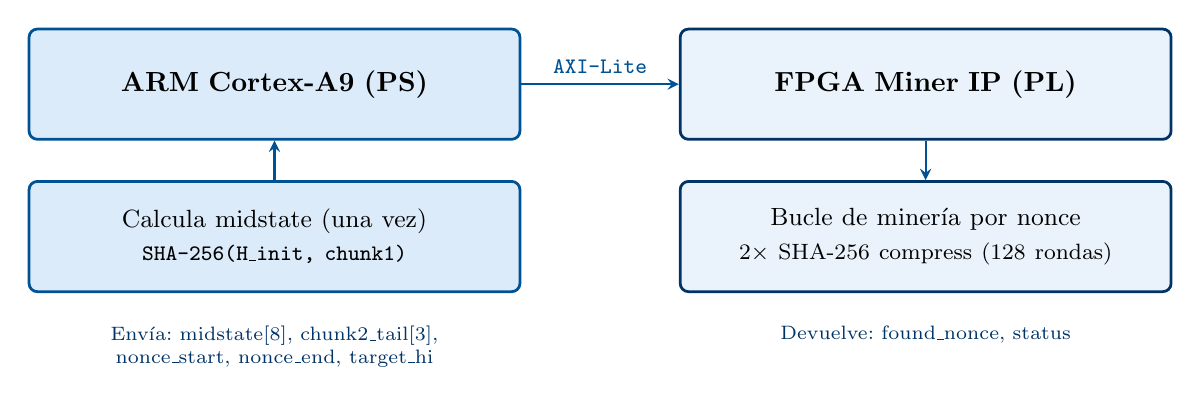
\begin{tikzpicture}[
    block/.style={rectangle, draw=medblue, fill=paleblue, text width=6cm,
        text centered, minimum height=1.4cm, rounded corners=3pt, line width=1pt},
    hwblock/.style={rectangle, draw=darkblue, fill=paleblue!60!white, text width=6cm,
        text centered, minimum height=1.4cm, rounded corners=3pt, line width=1pt},
    arrow/.style={->, thick, >=stealth, color=medblue}
]
    \node[block] (arm) {\textbf{ARM Cortex-A9 (PS)}};
    \node[block, below=0.5cm of arm] (midstate) {
        \small Calcula midstate (una vez) \\
        \footnotesize \texttt{SHA-256(H\_init, chunk1)}
    };
    \node[hwblock, right=2cm of arm] (fpga) {\textbf{FPGA Miner IP (PL)}};
    \node[hwblock, below=0.5cm of fpga] (mining) {
        \small Bucle de miner\'ia por nonce \\
        \footnotesize $2\times$ SHA-256 compress (128 rondas)
    };
    \draw[arrow] (arm) -- node[above, font=\footnotesize]{\texttt{AXI-Lite}} (fpga);
    \draw[arrow] (midstate) -- (arm);
    \draw[arrow] (fpga) -- (mining);
    \node[below=0.3cm of midstate, text width=6cm, align=center, font=\scriptsize\color{darkblue}] {
        Env\'ia: midstate[8], chunk2\_tail[3], \\
        nonce\_start, nonce\_end, target\_hi
    };
    \node[below=0.3cm of mining, text width=6cm, align=center, font=\scriptsize\color{darkblue}] {
        Devuelve: found\_nonce, status
    };
\end{tikzpicture}
\end{center}

% =============================================================================
\section{Arquitectura del Sistema}
% =============================================================================

\subsection{Interfaz del IP HLS}

La firma de la funci\'on HLS del IP es:

\begin{lstlisting}[style=cstyle]
void pico_miner(
    unsigned int midstate[8],      // Estado SHA-256 precalculado (midstate)
    unsigned int chunk2_tail[3],   // merkle_tail, timestamp, bits
    unsigned int nonce_start,      // Inicio del rango de nonces
    unsigned int nonce_end,        // Fin del rango (exclusivo)
    unsigned int target_hi,        // MSB del objetivo de dificultad
    unsigned int *found_nonce,     // Salida: nonce encontrado
    unsigned int *status           // Salida: 1 = encontrado, 0 = no encontrado
);
\end{lstlisting}

Todos los puertos se mapean a AXI-Lite (\texttt{s\_axilite}) agrupados en un
bus llamado \texttt{myaxi}. Vivado HLS 2019.1 mapea los argumentos de tipo array
como registros escalares individuales:
\begin{itemize}[leftmargin=2em]
    \item \texttt{midstate[8]} $\rightarrow$ \texttt{Set\_midstate\_0} \ldots \texttt{Set\_midstate\_7}
    \item \texttt{chunk2\_tail[3]} $\rightarrow$ \texttt{Set\_chunk2\_tail\_0} \ldots \texttt{Set\_chunk2\_tail\_2}
\end{itemize}

\subsection{Interfaz de Registros AXI-Lite}

\begin{table}[h]
    \centering
    \caption{Registros AXI-Lite}
    \rowcolors{2}{paleblue}{white}
    \begin{tabular}{@{}lll@{}}
        \toprule
        \textbf{Direcci\'on} & \textbf{Registro} & \textbf{Funci\'on del Driver SDK} \\
        \midrule
        Entrada  & midstate[0..7]     & \texttt{XPico\_miner\_Set\_midstate\_0} .. \texttt{\_7} \\
        Entrada  & chunk2\_tail[0..2] & \texttt{XPico\_miner\_Set\_chunk2\_tail\_0} .. \texttt{\_2} \\
        Entrada  & nonce\_start       & \texttt{XPico\_miner\_Set\_nonce\_start} \\
        Entrada  & nonce\_end         & \texttt{XPico\_miner\_Set\_nonce\_end} \\
        Entrada  & target\_hi         & \texttt{XPico\_miner\_Set\_target\_hi} \\
        Salida   & found\_nonce       & \texttt{XPico\_miner\_Get\_found\_nonce} \\
        Salida   & status             & \texttt{XPico\_miner\_Get\_status} \\
        \bottomrule
    \end{tabular}
\end{table}

\subsection{Flujo de Operaci\'on de Miner\'ia}

\begin{enumerate}[leftmargin=2em]
    \item El ARM analiza la cabecera de 80 bytes y la convierte a big-endian
    \item El ARM calcula el midstate: \texttt{sha256\_compress(H\_init, chunk1)}
    \item El ARM escribe midstate[8], chunk2\_tail[3], rango de nonces y target en la FPGA v\'ia AXI-Lite
    \item El ARM env\'ia \texttt{ap\_start}
    \item La FPGA itera nonces:
    \begin{enumerate}
        \item Construye el bloque de mensaje del chunk 2 (tail + nonce + relleno SHA-256)
        \item Comprime chunk 2 con el midstate $\rightarrow$ primer hash
        \item Hashea el primer hash con valores iniciales SHA-256 $\rightarrow$ hash final
        \item Si \texttt{final\_hash[7] <= target\_hi}: almacena nonce, establece status
    \end{enumerate}
    \item El ARM sondea \texttt{ap\_done}, luego lee \texttt{found\_nonce} y \texttt{status}
\end{enumerate}

\subsection{Estrategia de Miner\'ia por Fragmentos}

Para la demostraci\'on, el driver ARM divide la b\'usqueda completa de nonces en
fragmentos (\textit{chunks}) de 1.000.000 de nonces por invocaci\'on del hardware.
Entre fragmentos, el ARM:
\begin{itemize}[leftmargin=2em]
    \item Imprime el progreso (nonces buscados, porcentaje, tiempo transcurrido, tasa de hash) por UART
    \item Actualiza la barra de progreso de LEDs (8 LEDs del ZedBoard se encienden proporcionalmente)
    \item Comprueba si la FPGA ha encontrado un nonce v\'alido
\end{itemize}

Esto proporciona retroalimentaci\'on en tiempo real durante los $\sim$3 minutos de miner\'ia.

\subsection{Control de LEDs}

Los 8 LEDs del ZedBoard se controlan mediante un bloque AXI GPIO:
\begin{itemize}[leftmargin=2em]
    \item \textbf{Durante la miner\'ia}: Los LEDs se encienden proporcionalmente al progreso de b\'usqueda (0--8 LEDs)
    \item \textbf{Al completar}: Los 8 LEDs se encienden cuando el bloque se ha minado con \'exito
    \item \textbf{Animaci\'on de inicio}: Doble parpadeo de todos los LEDs al comenzar la miner\'ia
\end{itemize}

El driver utiliza \texttt{XGpio\_DiscreteWrite()} con \texttt{XPAR\_AXI\_GPIO\_0\_DEVICE\_ID}.

% =============================================================================
\section{Estrategia de Optimizaci\'on HLS}
% =============================================================================

\subsection{Funci\'on de Compresi\'on SHA-256}

La funci\'on \texttt{sha256\_compress()} es el n\'ucleo computacional cr\'itico.
Las optimizaciones clave aplicadas son:

\begin{lstlisting}[style=cstyle]
static void sha256_compress(const unsigned int state_in[8],
                            const unsigned int W_in[16],
                            unsigned int state_out[8])
{
#pragma HLS INLINE off
    unsigned int W[64];
#pragma HLS ARRAY_PARTITION variable=W complete dim=1

    // Carga + expansion de W (completamente desenrollado)
    // 64 rondas de compresion (pipeline II=1)
    compress:
    for (i = 0; i < 64; i++) {
#pragma HLS PIPELINE II=1
        // ... calculo de ronda
    }
}
\end{lstlisting}

\begin{itemize}[leftmargin=2em]
    \item \texttt{ARRAY\_PARTITION complete} en \texttt{W[64]}: las 64 palabras accesibles en paralelo (sin contenci\'on de puertos de memoria)
    \item \texttt{UNROLL} en carga y expansi\'on de W: calculado combinacionalmente
    \item \texttt{PIPELINE II=1} en el bucle de 64 rondas: una ronda por ciclo de reloj
    \item \texttt{INLINE off}: mantiene la funci\'on compress como m\'odulo reutilizable (se llama dos veces por nonce)
\end{itemize}

\subsection{Bucle de Miner\'ia}

El bucle de miner\'ia de nivel superior no tiene pragma de pipeline expl\'icito.
Cada iteraci\'on llama a \texttt{sha256\_compress} dos veces secuencialmente,
por lo que cada nonce tarda aproximadamente $2 \times 64 = 128$ ciclos de reloj.

\subsection{Configuraciones de Soluci\'on}

\begin{table}[h]
    \centering
    \caption{Configuraciones de soluci\'on HLS}
    \rowcolors{2}{paleblue}{white}
    \begin{tabular}{@{}lccc@{}}
        \toprule
        \textbf{Soluci\'on} & \textbf{Compress II} & \textbf{Ciclos/nonce} & \textbf{Throughput} \\
        \midrule
        1: Baseline (II=1) & 1 & $\sim$128 & $\sim$780 KH/s \\
        2: Relaxed (II=2)  & 2 & $\sim$256 & $\sim$390 KH/s \\
        \bottomrule
    \end{tabular}
\end{table}

La Soluci\'on 2 utiliza una directiva Tcl para relajar el II=1 del c\'odigo fuente:

\begin{lstlisting}[style=tclstyle]
set_directive_pipeline -II 2 "sha256_compress/compress"
\end{lstlisting}

Esto proporciona m\'as margen de timing si la Soluci\'on 1 no cumple la restricci\'on
de 10\,ns a 100\,MHz.

% =============================================================================
\section{Bloque 939260 -- Demostraci\'on}
% =============================================================================

El bloque seleccionado para la demostraci\'on es el Bloque 939260 de Bitcoin,
minado el 4 de marzo de 2026. Sus caracter\'isticas lo hacen apropiado para
una demostraci\'on en clase:

\begin{table}[h]
    \centering
    \caption{Datos del Bloque 939260}
    \rowcolors{2}{paleblue}{white}
    \begin{tabular}{@{}ll@{}}
        \toprule
        \textbf{Campo} & \textbf{Valor} \\
        \midrule
        Altura                & 939.260 \\
        Fecha                 & 4 de marzo de 2026 \\
        Dificultad            & 144.398.401.518.101 \\
        Nonce (LE)            & \texttt{0x1E740A08} \\
        Nonce (BE)            & \texttt{0x080A741E} ($\sim$134,9M) \\
        Hash del bloque       & \texttt{00000000000000000001758847...} \\
        Tiempo estimado       & $\sim$3 min a 781 KH/s \\
        \bottomrule
    \end{tabular}
\end{table}

\textbf{Cabecera cruda} (hex, 80 bytes):

\texttt{\small 0000003c 3c08f14a ad5cac28 2d1c8ca8 79310a24 15794de3 8e4e0100}
\texttt{\small 00000000 00000000 fc9099f6 927218e1 2db0cc20 ef43657d 5a32cba9}
\texttt{\small 3b8994ba 59a61054 ddf1af1b bf28a869 03f30117 080a741e}

\textbf{Hash del bloque} (orden de visualizaci\'on):

\texttt{\small 000000000000000000017588478b3612182486d33006ede1164fb146fa41cd06}

\subsection{Orden de Bytes del Nonce}

Bitcoin serializa los nonces en \textbf{little-endian} (LE) en la cabecera del bloque.
SHA-256 procesa palabras en \textbf{big-endian} (BE). La FPGA itera directamente la
palabra de nonce en BE. La FPGA busca en un orden diferente a un minero LE, pero
cubre el mismo espacio de $2^{32}$ nonces y produce hashes id\'enticos para cualquier
valor de nonce dado.

% =============================================================================
\section{Verificaci\'on y Pruebas}
% =============================================================================

\subsection{Testbench HLS (5 Pruebas)}

El testbench (\texttt{pico\_miner\_tb.cpp}) contiene cinco casos de prueba:

\begin{table}[h]
    \centering
    \caption{Casos de prueba del testbench}
    \rowcolors{2}{paleblue}{white}
    \begin{tabular}{@{}clp{8cm}@{}}
        \toprule
        \textbf{Test} & \textbf{Tipo} & \textbf{Descripci\'on} \\
        \midrule
        1 & Vector NIST    & SHA-256(``abc'') validado contra FIPS 180-4 \\
        2 & Bloque 1 SW    & Miner\'ia completa desde nonce=0 ($\sim$31,8M iteraciones) en software \\
        3 & Bloque 1 HW    & Acelerador HLS con ventana $\pm16$ nonces \\
        4 & Bloque 939260 HW & Acelerador HLS con ventana $\pm16$ nonces \\
        5 & Sin soluci\'on  & Verifica que el acelerador reporta ``no encontrado'' \\
        \bottomrule
    \end{tabular}
\end{table}

Las ventanas estrechas de $\pm16$ nonces para las pruebas HW mantienen la
co-simulaci\'on C/RTL r\'apida (32 nonces $\times$ 128 ciclos/nonce $\approx$
4096 ciclos por bloque). La b\'usqueda completa en el Test 2 se ejecuta en
software puro para evitar timeouts en la co-simulaci\'on.

\subsection{Simulaci\'on C (csim)}

Las cinco pruebas se ejecutan durante \texttt{csim\_design}. La b\'usqueda completa
del Bloque 1 (Test 2) tarda $\sim$10 segundos en simulaci\'on C.

\subsection{Co-Simulaci\'on C/RTL (cosim)}

Tras la s\'intesis C, el RTL generado se verifica contra el testbench C.
Las llamadas HW usan ventanas estrechas de nonces ($\pm16$) para mantener
el tiempo de co-simulaci\'on manejable.

\subsection{Verificaci\'on en ARM}

El driver ARM (\texttt{pico\_miner\_arm.c}) mina el Bloque 939260 en hardware FPGA
mediante b\'usqueda completa desde nonce=0. Tras encontrar un nonce, el ARM:
\begin{enumerate}[leftmargin=2em]
    \item Ejecuta el modelo dorado SW (double-SHA-256 completo) sobre el nonce encontrado
    \item Muestra el hash calculado en orden de visualizaci\'on de Bitcoin
    \item Compara el nonce encontrado con el nonce conocido de la blockchain
    \item Informa del estado de verificaci\'on por terminal UART
\end{enumerate}

% =============================================================================
\section{Resultados}
% =============================================================================

\subsection{Rendimiento Estimado}

A 100 MHz con compresi\'on II=1, la latencia de compresi\'on SHA-256 es de 64 ciclos.
Cada nonce requiere dos compresiones, resultando en $\sim$128 ciclos por nonce:
\[
    \text{Throughput} = \frac{100 \times 10^6 \text{ ciclos/s}}{128 \text{ ciclos/nonce}}
    \approx 781.250 \text{ H/s} \approx 781 \text{ KH/s}
\]

\subsection{Tiempo de Miner\'ia del Bloque 939260}

El nonce BE del Bloque 939260 es \texttt{0x080A741E} ($\approx$134,9M).
A $\sim$781 KH/s:
\[
    \text{Tiempo} = \frac{134.900.000}{781.000} \approx 172,7 \text{ s}
    \approx 2 \text{ min } 53 \text{ s}
\]

Esto constituye un tiempo de demostraci\'on apropiado para el aula.

\subsection{Comprobaci\'on de Dificultad}

El hash del Bloque 939260 comienza con 19 ceros hexadecimales (76 bits a cero)
en orden de visualizaci\'on. La comprobaci\'on simplificada \texttt{final\_hash[7] == 0}
verifica que los primeros 32 bits en orden de visualizaci\'on son cero. Aunque esto
es menos restrictivo que la dificultad real (que requiere 76+ bits a cero), es
suficiente para la demostraci\'on. La probabilidad de un falso positivo
(\texttt{final\_hash[7] == 0} para un nonce aleatorio) es $1/2^{32} \approx$
2,3 $\times 10^{-10}$, acumulando $\sim$3\% sobre los 134,9M nonces buscados.

% =============================================================================
\section{Gu\'ia de Reproducci\'on}
% =============================================================================

\subsection{Paso 1: Vivado HLS}

Sintetizar el IP de miner\'ia:

\begin{lstlisting}[style=tclstyle]
vivado_hls -f run_hls.tcl
\end{lstlisting}

Alternativamente, en la GUI de Vivado HLS:
\begin{enumerate}[leftmargin=2em]
    \item Crear nuevo proyecto, funci\'on top \texttt{pico\_miner}
    \item A\~nadir \texttt{src/pico\_miner.cpp} y \texttt{src/pico\_miner.h} como archivos fuente
    \item A\~nadir \texttt{src/pico\_miner\_tb.cpp} como testbench
    \item Establecer dispositivo objetivo: \texttt{xc7z020clg484-1}, reloj: 10\,ns (100 MHz)
    \item Ejecutar C Simulation $\rightarrow$ debe mostrar ``ALL TESTS PASSED (5 tests)''
    \item Ejecutar C Synthesis $\rightarrow$ genera RTL + informe de rendimiento
    \item Ejecutar C/RTL Co-Simulation $\rightarrow$ verifica que el RTL coincide con el comportamiento C
    \item Exportar RTL (formato IP Catalog)
\end{enumerate}

\subsection{Paso 2: Vivado -- Dise\~no de Bloques}

\begin{enumerate}[leftmargin=2em]
    \item Abrir Vivado 2019.1, crear proyecto para \texttt{xc7z020clg484-1}
    \item Crear un Block Design
    \item A\~nadir el IP \textbf{ZYNQ7 Processing System}
    \item A\~nadir el IP \textbf{Pico Miner} (desde la exportaci\'on HLS)
    \item A\~nadir un IP \textbf{AXI GPIO}, configurar como salida de 8 bits (LEDs)
    \item Mantener \texttt{FCLK\_CLK0 = 100 MHz} (por defecto)
    \item Ejecutar \textbf{Connection Automation}
    \item Conectar la salida GPIO a los pines de LED del ZedBoard (restricciones XDC)
    \item Generar bitstream
    \item Exportar Hardware (incluir bitstream) y lanzar SDK
\end{enumerate}

\subsection{Paso 3: Xilinx SDK}

\begin{enumerate}[leftmargin=2em]
    \item Crear un nuevo Application Project (plantilla \textbf{Empty Application})
    \item A\~nadir \texttt{src/pico\_miner\_arm.c} a la carpeta \texttt{src/}
    \item Compilar el proyecto
    \item Programar la FPGA y ejecutar la aplicaci\'on
    \item Observar resultados en el terminal serie UART (115200 baudios)
    \item Observar los LEDs del ZedBoard encendi\'endose progresivamente
\end{enumerate}

\textbf{Nota}: Usar la plantilla ``Empty Application'', no ``Hello World''.
El driver usa \texttt{xil\_cache.h} directamente (no \texttt{platform.h}).

% =============================================================================
\section{Conclusi\'on}
% =============================================================================

Pico Miner demuestra la miner\'ia Bitcoin double-SHA-256 con optimizaci\'on de midstate
en una FPGA Zynq-7020 mediante Vivado HLS 2019.1. El sistema realiza una b\'usqueda
por fuerza bruta del Bloque 939260 (4 de marzo de 2026, dificultad
144.398.401.518.101) desde nonce=0, encontrando el nonce correcto en
aproximadamente 3 minutos.

El dise\~no se verifica a m\'ultiples niveles:
\begin{itemize}[leftmargin=2em]
    \item Validaci\'on contra vector de prueba NIST FIPS 180-4
    \item Miner\'ia completa del Bloque 1 desde nonce=0 ($\sim$31,8M iteraciones) en software
    \item Miner\'ia hardware de los Bloques 1 y 939260 con comparaci\'on bit-exacta SW/HW
    \item Hashes de bloque verificados contra la blockchain
    \item Verificaci\'on SW del nonce encontrado por hardware en el driver ARM
\end{itemize}

El proyecto demuestra:
\begin{itemize}[leftmargin=2em]
    \item S\'intesis de Alto Nivel (HLS) de SHA-256 desde C hasta RTL
    \item Optimizaci\'on de midstate para partici\'on de trabajo ARM/FPGA
    \item Integraci\'on AXI-Lite para comunicaci\'on PS/PL
    \item Optimizaci\'on mediante directivas HLS (pipeline II=1, partici\'on de arrays, desenrollamiento)
    \item Control de GPIO para retroalimentaci\'on visual (LEDs)
    \item Medici\'on de rendimiento en tiempo real (XTime)
\end{itemize}

El throughput estimado es de $\sim$781\,KH/s a 100\,MHz con compresi\'on II=1
($\sim$128 ciclos por nonce).

% =============================================================================
\section{Archivos del Proyecto}
% =============================================================================

\begin{table}[h]
    \centering
    \caption{Archivos del proyecto}
    \rowcolors{2}{paleblue}{white}
    \begin{tabular}{@{}lp{9cm}@{}}
        \toprule
        \textbf{Archivo} & \textbf{Descripci\'on} \\
        \midrule
        \texttt{src/pico\_miner.h}      & Constantes SHA-256 (H0-H7, K[64]), prototipo de funci\'on, defines de interfaz \\
        \texttt{src/pico\_miner.cpp}    & Fuente HLS: \texttt{sha256\_compress()} + bucle de miner\'ia double-SHA-256 con midstate \\
        \texttt{src/pico\_miner\_tb.cpp} & Testbench HLS: 5 pruebas (NIST, Bloque 1 SW+HW, Bloque 939260 HW, sin soluci\'on) \\
        \texttt{src/pico\_miner\_arm.c}  & Driver ARM: demo Bloque 939260 con progreso, LEDs, XTime \\
        \texttt{doc/memoria\_es.tex}    & Este documento (versi\'on en espa\~nol) \\
        \texttt{doc/memory\_en.tex}     & Memoria del proyecto (versi\'on en ingl\'es) \\
        \texttt{run\_hls.tcl}           & Script TCL: 2 soluciones (II=1, II=2), csim/csynth/cosim/export \\
        \bottomrule
    \end{tabular}
\end{table}

% =============================================================================
\end{document}
